\documentclass[]{article}

\author{Kelsey Iafrate}
\title{Homework 3}

\usepackage{geometry}

\geometry{margin=1in}
\usepackage{Sweave}
\begin{document}

\maketitle

\Sconcordance{concordance:Homework3.tex:Homework3.Rnw:%
1 8 1 1 0 81 1 1 2 1 0 3 1 4 0 1 3 1 0 2 1 4 0 1 2 8 1 1 2 1 0 3 1 6 0 %
1 2 3 1 1 2 7 0 1 2 5 1}



\begin{enumerate}

\item 
The expected value of $Y_i$ is not the model, and it would not include $\epsilon _i$. The student should have written Y=$\beta _0$ + $\beta _1$

\item
The mistake the researchers made was assuming that the correlation between exercise frequency and cold frequency was caused by the change in exercise frequency. Correlation does not imply causation.  

\item
Finding the least squares does not depend on $\epsilon$ being normally distributed. The normality of $\epsilon$ is important for finding the distribution of Y. It ensures the line is an unbiased estimator for Y and the estimated coefficients are unbiased for the true regression coefficients. 

\item
For the special case where $\beta _0$ = 0, the minimum SSE for $\beta _1$ is the minimum of
  
  \begin{center} $\Sigma (y_i-\hat{y_i})^2$ = $\Sigma (y_i - \beta _1x_i)^2$
  
  We take the derivative with respect to $\beta _0$ and set it equal to zero to get
  
  $-2\Sigma x_i(y_i-\beta  _1x_i) = 0 ,$
  
  $equal\ to\ \Sigma(y_ix_i-\beta _1x_i^2) = 0,$
  
  $equal\ to\ \beta _1 = \frac{\Sigma x_iy_i}{\Sigma x_i^2}.$
  \end{center}
  
\item 
For the special case where $\beta _1$ = 0, the minimum SSE for $\beta _0$ is the minimum of
  \begin{center} $\Sigma(y_i-\hat{y_i})^2 = \Sigma (y_i - \beta _0)^2$
  
  We take the derivative with respect to $\beta _0$ and set it equal to zero to get
  
  $-2\Sigma(y_i-\beta _0) = 0 ,$
  
  $equal\ to\ \Sigma (y_i) - n\beta _0 =0,$
  
  $equal\ to\ \beta _0 = \frac{\Sigma y_i}{n}=\bar{y}$.
  
 \end{center}
 
 This makes sense since if there is no linear relation between X and Y, then we would expect the expected value of Y to be as if we were just drawing a random sample of Y where E(Y)=$\bar{y}.$

\item
For the simple linear regression model $Y=\beta _0 + \beta _1 X + \epsilon$ ,
since $\hat{\beta _0} = \bar{y}-\hat{\beta}\bar{x},$

\begin{center}
$E{\hat{\beta _0}}=E(\bar{y}-\hat{\beta}\bar{x})= E(\bar{y})-E(\hat{\beta}\bar{x}).$

Since $\bar{x}$ is constant, $E(\bar{y})=\beta _0 + \beta _1 \bar{x}$, and $\hat{\beta}_1$ is unbiased for $\beta _1,$ 

$E(\hat{\beta _0})=\beta _0 +\beta _1 \bar{x}-\beta _1 \bar{x} = \beta _0.$

\end{center}

Therefore, $\hat{\beta _0}$ is an unbiased estimator of $\beta _0$
\item

Assume the $i^{th}$ observation falls exactly on the regression line. If we reorder the data such that the $i^{th}$ observation is now the $n^{th}$ observation, we see $$SSE = \sum_{i=1}^{n}(y_i-\hat{y}_i)$$ $$=(y_n-\hat{y}_n)+\sum_{i=1}^{n-1}(y_i-\hat{y}_i).$$ Since $y_n$ is on the line, $y_n$ = $\hat{y}_n$, so $$SSE =\sum_{i=1}^{n-1}(y_i-\hat{y}_i).$$

Therefore, if we simply remove the point on the line, the SSE from which we derive our regression coefficients will be unchanged. Thus removing the point will not change the least squares line fitted to the remaining n-1 observations.

\item
Since the p-value for the estimated slope is huge (.91), we fail to reject the hypothesis that there is no linear relationship between sales and advertising. Therefore, we may not interpret the slope.

\item
The precision of the model depends not only on the value of $R^2$, but on the regression statistics as well. It is possible to have a high coefficient of determination, yet have regression coefficients that indicated no linear relationship. If, however, the regression coefficients, specifically that of the slope, indicated a linear relationship between the independent and dependent variables, then, by definition, an $R^2$ close to 1 implies the model is precise in predicting Y. 

\item

\begin{enumerate}
\item
If the variance of $\epsilon$ increases as X increases, there is not a linear relationship between X and Y in the range presented by the data. It is possible that a subset of X would produce a linear relationship. For example if we had data from independent movie box office sales versus DVDs sold mixed in with blockbuster films, we may see an increase in variance as the box office sales increase. But as we saw in the example in class, there is a linear relationship between box office sales and DVD sales in just independent films.

\item
If the variance of $\epsilon$ increases as X increases, it is still possible that there is some association between X and Y. The relation could be something other than linear, such as logarithmic or hyperbolic. 
\begin{Schunk}
\begin{Sinput}
> X <- c(20:100)
> Y <- exp(X)
> linMod <- lm(Y~X)
> plot.lm(linMod,which=1)
\end{Sinput}
\end{Schunk}
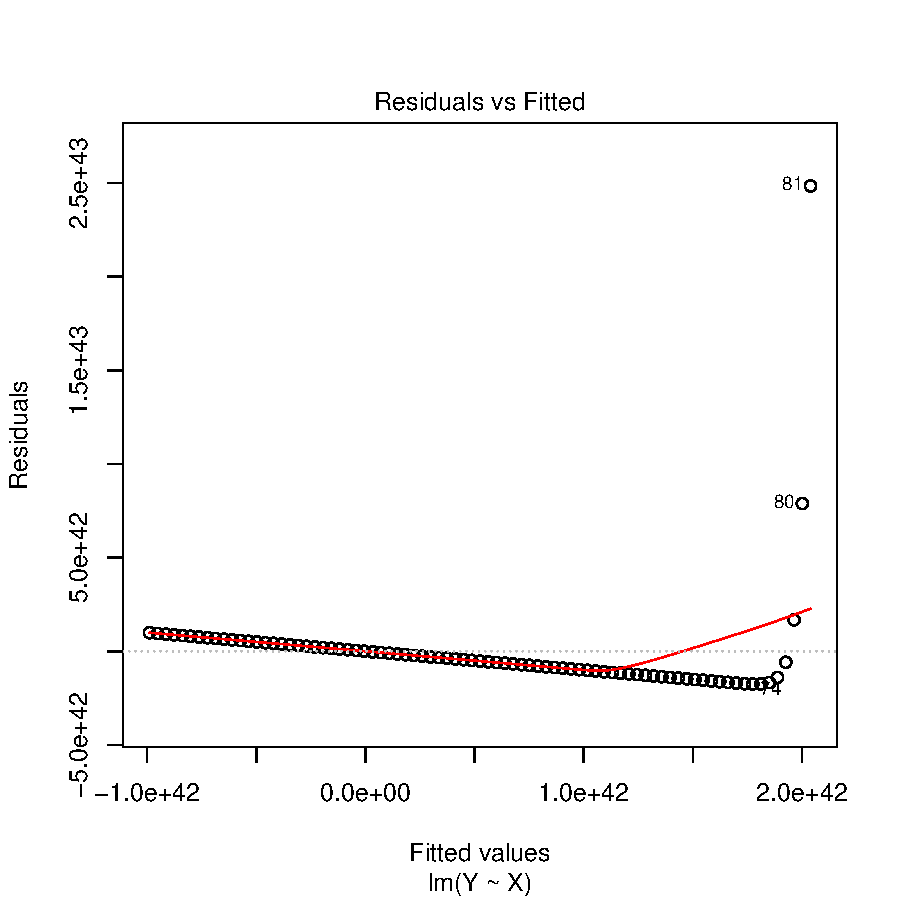
\includegraphics{Homework3-001}
\begin{Schunk}
\begin{Sinput}
> linMod2 <- lm(log(Y)~X)
> plot(X,log(Y))
> abline(linMod2)
\end{Sinput}
\end{Schunk}
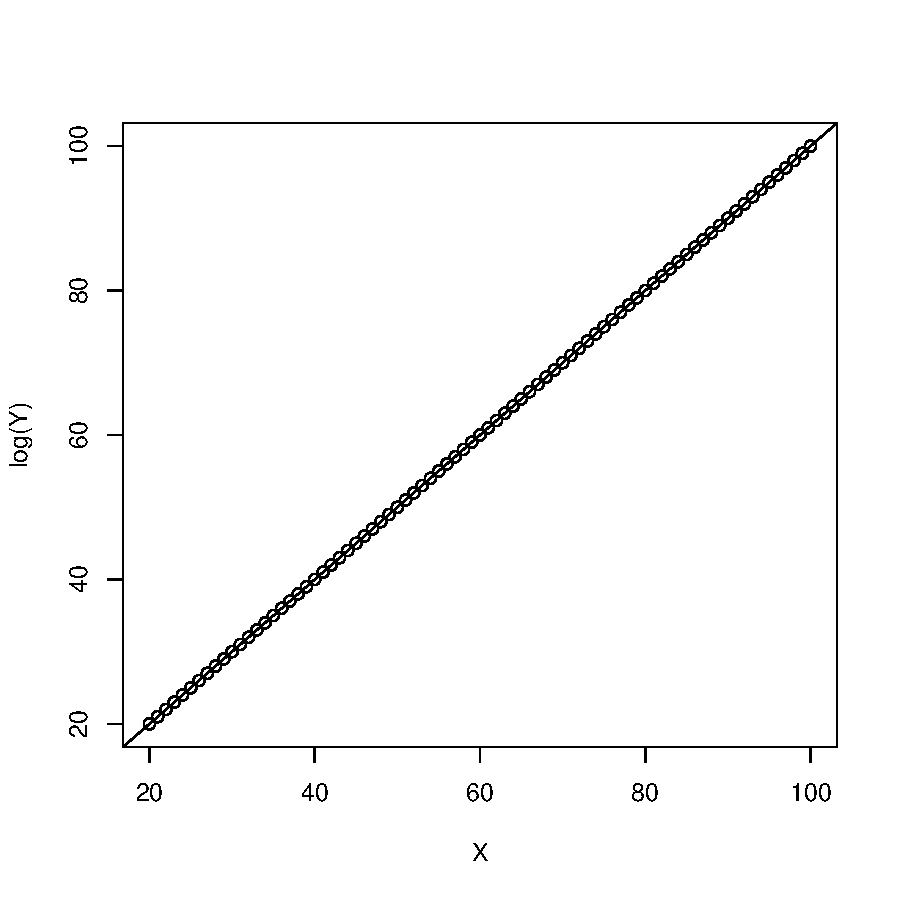
\includegraphics{Homework3-002}

As we can see in this example, when doing a simple linear regression on X and Y, the residuals get exponentially large as X gets large, which invalidated the constant variation of the residuals. However, there is a relationship between X and Y as seen when finding the linear regression of X and log(Y). 

\end{enumerate}

\item
We know E(MSE) = $\sigma ^2$ = $0.6^2$ = 0.36.

The MSR = SSR = $\Sigma (\hat{y}_i-\bar{y})^2$.
\begin{Schunk}
\begin{Sinput}
> X<-c(1,4,10,11,14)
> yBar <- 5 + 3*mean(X)
> yi<-5+3*X
> sum((yi-yBar)^2)
\end{Sinput}
\begin{Soutput}
[1] 1026
\end{Soutput}
\end{Schunk}

So the MSR = 1026.

I could not find anything about E(MSR) in the notes. Penn State's website on regression says E(MSR) = $\sigma ^2 + \beta _1^2 \Sigma(X_i-\bar{X})^2$=
\begin{Schunk}
\begin{Sinput}
> .36+9*sum((X-mean(X))^2)
\end{Sinput}
\begin{Soutput}
[1] 1026.36
\end{Soutput}
\end{Schunk}


\end{enumerate}


\end{document}
